\graphicspath{{./FirstTask/}} % path to graphics

\section*{\Large Цель практическои работы}
\addcontentsline{toc}{section}{Цель практическои работы}

\textbf{Цель работы} --- изучить структуру и функционал рассматриваемой
информационной системы, освоить правила посторения диаграммы вариантов
использования.

\textbf{Задачи:}\par
\begin{itemize}
	\item изучить предметную область по заданным вариантам;
	\item определить на концептуальном уровне состав элементов системы;
	\item описать функции рассматриваемой системы с помощью диаграммы 
		вариантов использования.
\end{itemize}
\newpage

\section{Анализ существующих сайтов}
\subsection{Аптека 36.6}

\textbf{Достоинства:}\par
\begin{itemize}
	\item есть поисковая строка;
	\item есть регистрация;
	\item есть возможность помечать товары как избранные;
	\item товар разбит на категории, такие как:
	\begin{itemize}
		\item выгодно;
		\item лекарства;
		\item витамины и БАДы;
		\item косметика;
		\item гигиена;
		\item уход за больными;
	\end{itemize}
	\item есть программа лояльности;
	\item есть меню с инструкцией, как заказать товар;
\end{itemize}

\textbf{Недостатки:} нет выбора товара по производителю,
нет возможности сортировки товара по производителю,
нет возможности выбора товара по сроку годности,
нет возможности выбора товара по наличию.

\subsection{Горздрав}
\textbf{Достоинства:}\par
\begin{itemize}
	\item возможность поиска товара по алфавиту;
	\item есть регистрация;
	\item есть возможность помечать товары как избранные;
	\item товар разбит на категории, такие как:
	\item вкладка со скидками и акциями
\end{itemize}

\textbf{Недостатки:} нет возможности выбора товара по производителю,
нет оформить подписку на ежемесечную доставку товара. Также поля для получения информации о стадии выполнения заказов.

\section{Основные необходимы функции}
На основе проведнного исследования предметной области были выделены основные
функции, которые должна выполнять система. Эти функции будут использоваться
при построении диаграммы вариантов использования.

\textbf{Функции:}
\begin{itemize}
	\item Поиск товара (фильтры): по названию; по алфавиту; по производителю;
		по сроку годности; по наличию; по категории; по цене; по рейтингу;
	\item Возможность оформить ежемесячную подписку на доставку товара;
	\item Регистрация личного кабинета для сохранния истории заказов;
	\item Поле для получения информации о стадии выполнения заказов;
	\item Возможность пометить товар как избранный;
	\item Поле для оставления отзывов о товаре;
	\item База данных, хранящая информацию о клиентах (ФИО, телефон и др.);
	\item Программа лояльности;
	\item Страницы с различной информацией по теме сайта;
	\item Страницы с инструкцие по заказу товаров;
	\item Возможность выбирать способы оплаты;
	\item Доставка заказанного товара;
\end{itemize}

На основе выделеных функций опишем решение
в виде таблицы \ref{table:desc_of_elements}.
\begin{table}[h!tp]
	\caption{\leftline{Описание элементов}}
	\label{table:desc_of_elements}
	\begin{tabular}{|p{0.25\textwidth}|p{0.70\textwidth}|}
		\hline Наименование & Краткое описание\\ \hline
		Выбор товара & Поиск товара(фильтры).\par
			Возможность пометить товар как избранный.\\ \hline
		Регистрации & Регистрация личного
			кабинета для сохранния истории заказов.\\ \hline
		Обратный отклик & Поле для оставления отзывов о товаре.\\ \hline
		Подписка & Программа лояльности.\par
			Возможность оформить ежемесячную
			подписку на доставку товара.\\ \hline
		Предоставление информации & Страницы с различной информацией
			по теме сайта.\par Страницы с инструкцие по заказу товаров.\par
			Поле для получения информации о стадии выполнения заказов.\\ \hline
		Сохранение данных о пользователях & База данных, хранящая информацию
			о клиентах (ФИО, телефон и др.).\\ \hline
		Оплата & Возможность выбирать способы оплаты\\ \hline
		Доставка & Доставка заказанного товара.\\ \hline
	\end{tabular}
\end{table}

\section{Ожидаемые результаты реализации}
По итогу, ожидаемые результаты реализации моделируемой
системы включают: уменьшение времени поиска товара,
увеличение количества привлеченных клиентов, увеличение прибыли, 
уменьшение скорости предоставления нужной информации.


\section{Диаграмму вариантов использования}
На основе выделеных основных вариантов использования (функций) системы
спроектируем диаграму вариантов использования
(Рисунок~\ref{fig:use_case_diagram}). А затем
для каждого из них построить диаграммы декомпозиции (детализации). 
Также нужно учесть какие активные субъекты должны взаимодействовать с
будущей системой.

\begin{figure}[h!tp]
	\centering
	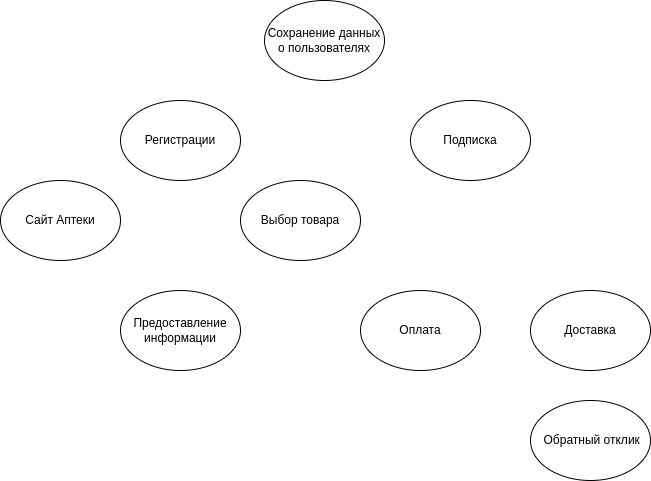
\includegraphics[width=0.7\textwidth]{use_case_diagram}
	\caption{Диаграмма вариантов использования}
	\label{fig:use_case_diagram}
\end{figure}

\newpage
Далее, добавим к деаграмме актеров
(Рисунок~\ref{fig:use_case_diagram_with_acter}).

\begin{figure}[h!tp]
	\centering
	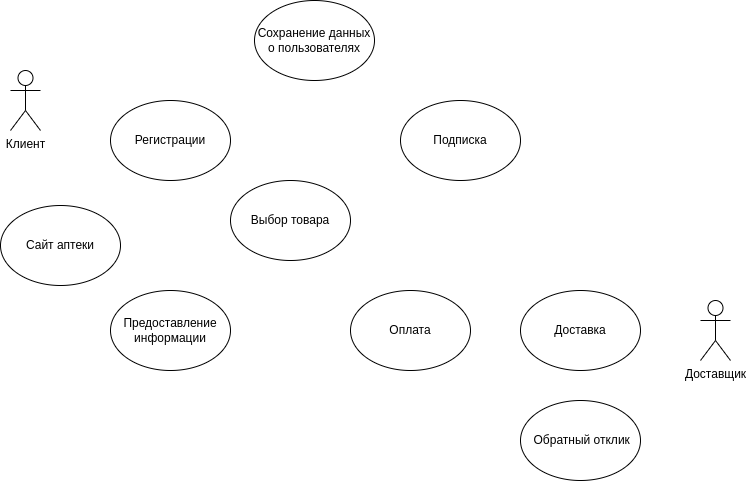
\includegraphics[width=0.7\textwidth]{use_case_diagram_with_acter}
	\caption{Диаграмма вариантов использования}
	\label{fig:use_case_diagram_with_acter}
\end{figure}

Теперь можно рассатвить связи между элемнтами,
как показанно на рис.~\ref{fig:use_case_complite}.

\begin{figure}[h!tp]
	\centering
	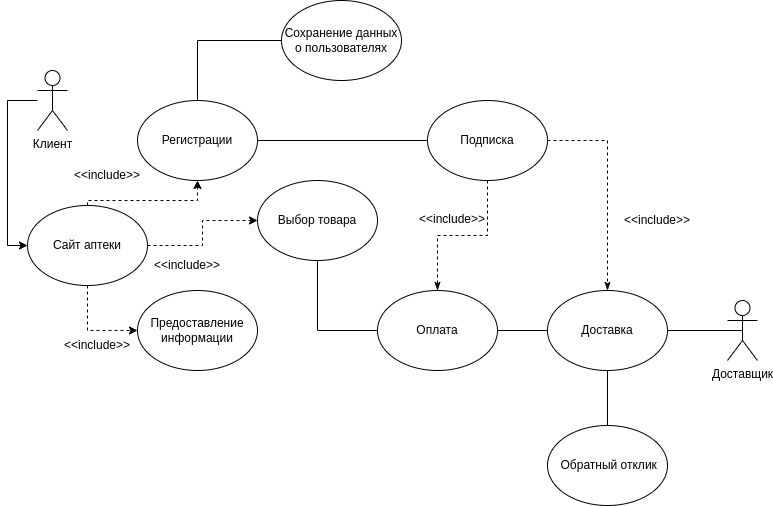
\includegraphics[width=0.7\textwidth]{use_case_complite}
	\caption{Диаграмма вариантов использования}
	\label{fig:use_case_complite}
\end{figure}

\newpage

\section*{Ответы на вопросы}
\addcontentsline{toc}{section}{Ответы на вопросы}

\begin{enumerate}
	\item \textbf{Для чего используется язык UML?}\par
		UML является языком широкого профиля, это --- открытый стандарт,
		использующий графические обозначения для создания абстрактной
		модели системы, называемой UML-моделью. UML был создан для
		\textbf{\textit{определения, визуализации, проектирования
		и документирования}}, в основном, программных систем. UML не является
		языком программирования, но на основании UML-моделей возможна
		генерация кода.
	\item \textbf{Какие диаграммы входят в состав языка UML?}\par
		Диаграмма активности, диаграмма классов, диаграмма последовательности,
		диаграмма состояний, диаграмма компонентов и диаграмма действий.
	\item \textbf{В чем смысл варианта использования?}\par
		Описывает, какой функционал разрабатываемой программной
		системы доступен каждой группе пользователей.
	\item \textbf{Каково назначение диаграмм вариантов использования.}\par
		Главное назначение диаграммы вариантов использования заключается
		в \textbf{\textit{формализации функциональных требований к системе}}
		с помощью понятий соответствующего пакета и возможности согласования
		полученной модели с заказчиком на ранней стадии проектирования.
	\item \textbf{Назовите основные свойства вариантов использования.}\par
		\begin{itemize}
			\item Вариант использования должен быть независимым от других
				вариантов использования.
			\item Вариант использования должен быть независимым от реализации.
			\item Вариант использования должен быть независимым от внешнего
				вида.
			\item Вариант использования должен быть независимым от технологии
				реализации.
		\end{itemize}
	\item \textbf{Назовите основные компоненты диаграмм вариантов
		использования.}\par
		\begin{itemize}
			\item Участник
			\item Варианты использования
			\item Ненаправленная ассоциация
			\item Направленная ассоциация
			\item Обобщение
			\item Зависимость
			\item Точка изгиба связей
			\item Комментарий
			\item Коннектор комментария
		\end{itemize}
	\item \textbf{Что такое «действующее лицо»?}\par
		Под действующим лицом или актер понимается любой объект,
		субъект или система, взаимодействующая с моделируемой системой извне.
	\item \textbf{Какую роль могут играть действующие лица по отношению
		к варианту использования?}\par
		Действующие лица представляют не физических людей или системы,
		а их роли. Это означает, что когда человек взаимодействует
		с системой различными способами (предполагая различные роли),
		он отображается несколькими действующими лицами.
		Например, человек, работающий в службе поддержки и принимающий
		от клиентов заказы, будет отображаться в системе как
		«участник отдела поддержки» и «участник отдела продаж».\par
		Действующие лица могут иметь два типа связей с вариантами
		использования: Простая ассоциация --- отражается линией между
		актером и вариантом использования (без стрелки).
		Отражает связь актера и варианта использования. простая ассоциация
		Направленная ассоциация --- то же что и простая ассоциация,
		но показывает, что вариант использования инициализируется актером.
		Обозначается стрелкой.
	\item \textbf{Каким образом анализ внешних событий позволяет определить
		варианты использования системы?}\par
		После анализа существующих на рынке решений и сбора информации
		производится вывод о том, что можно было бы добавить, или исключить
		в системе. Далее производится выделение основных функции реализуемой
		системы, которые становятся её вариантами.
	\item \textbf{Что позволяют получить диаграммы
		вариантов использования?}\par
		Диаграммы вариантов использования позволяют:
		\begin{itemize}
			\item определить общие границы и контекст моделируемой
				предметной области;
			\item сформулировать общие требования к функциональному поведению
				проектируемой системы;
			\item разработать исходную концептуальную модель системы для ее
			\item последующей детализации в форме логических
				и физических моделей;
			\item подготовить исходную документацию для взаимодействия
				разработчиков системы с ее заказчиками и пользователями.
		\end{itemize}
	\item \textbf{Что показывает диаграмма вариантов использования?}\par
		Диаграмма вариантов использования описывает какой функционал
		разрабатываемой программной системы доступен каждой группе
		пользователей. (описывает функциональное назначение системы)
	\item \textbf{Какие элементы содержит диаграмма
		вариантов использования?}\par
		Диаграмма вариантов использования \textit{состоит} из актеров,
		для которых система производит действие, и собственно действия
		Use Case, которое описывает то, что актер хочет получить от системы.
		Дополнительно в диаграммы могут быть добавлены комментарии
	\item \textbf{Что служит хорошим источником для идентификации
		вариантов использования?}\par
		Хорошим источником для идентификации вариантов использования
		служат внешние события. Стоит начинать с перечисления всех событий,
		происходящих во внешнем мире, на которые система должна каким-либо
		образом реагировать. Идентификация событий, на которые необходимо
		реагировать, помогает выделить варианты использования.
	\item \textbf{Что такое актер?}\par
		\textbf{\textit{Актером}} (действующим лицом, актантом, актором)
		называется любой объект, субъект или система,
		взаимодействующая с моделируемой системой извне.
	\item \textbf{Перечислите типы актеров и расскажите
		об их особенностях.}\par
		Действующие лица могут быть первичными или вторичными.
		\textbf{Первичный~актер} --- это актер, который использует систему для
		достижения цели. Примеры использования документируют взаимодействия
		между системой и актерами для достижения целей первичного актера.
		\textbf{Вторичные~актеры} --- это актеры, которым система должна
		оказывать помощь для достижения целей основного субъекта.
		Первичные актеры инициируют взаимодействие с системой.
		Система обычно обращается за помощью к вторичным актерам.
	\item \textbf{Какие отношения возможны между актерами?}\par
		Обобщения, включения.
\end{enumerate}

\newpage

\section*{Вывод}
\addcontentsline{toc}{section}{Вывод}
В результате проделанной работы был проведен анализ предметной области,
а если конкретнее, работа аптеки.
Были выделены преимущества и недостатки конкурентных предложений.
На основе которых были определены основные функции, которые должна выполнять
система. Также были поставлены ожидаемые результаты.
И, в результате, была составлена диаграмма вариантов с актерами и связями.

\newpage

\begin{thebibliography}{0}
	\bibitem{1} \textit{Интернет-магазин аптеки 36.6}
		URL:~https://www.36.6.ru/
	\bibitem{2} \textit{Интернет-магазин аптеки Горздрав}
		URL:~https://gorzdrav.org/
\end{thebibliography}

